\graphicspath{{./design/}}

\chapter{Design}
% {{{
\label{cha:design}

% {{{

The goal of the visualisation aspect of the system is to provide a way to
easily interpret the molecular data. The visualisation techniques chosen either
support the compression aspect of the water compression system, or allows for
general interpretation of data. The main challenge to the effective
visualisation of the data is the large amounts of visible clutter.

A brief overview of the entire system is provided in Section
\ref{sec:design_overview}, while Section \ref{sec:design_visualisation} provides
more detail into the visualisation components of the system.

% }}}

\section{System overview}
% {{{
\label{sec:design_overview}

The design of the system has been broken down into a number of components. The
most notable components are:

\begin{itemize}
  \item Quantiser - quantises and dequantises the data
  \item I/O - handles input and output of data
  \item Water cluster extractor - extracts the water clusters
  \item Verifiers - verify and record various aspects of the compression system
  \item Arithmetic coders - encodes and decodes symbols
  \item Visualisation - displays the simulation data
  \item Compressors - drivers behind the compression system
\end{itemize}

See Figure \ref{fig:design_overview} for a schematic diagram of the components
listed above. Julian Kenwood has completed the green areas, Keegan Smith has
completed the cyan areas, while I have completed the red areas. The Quantiser,
I/O and Water cluster extractor components are used by both the compressors and
the visualisation. The Verifiers and Arithmetic coder components are used by the
compressors only.

\begin{figure}[h!]
  \begin{center}
    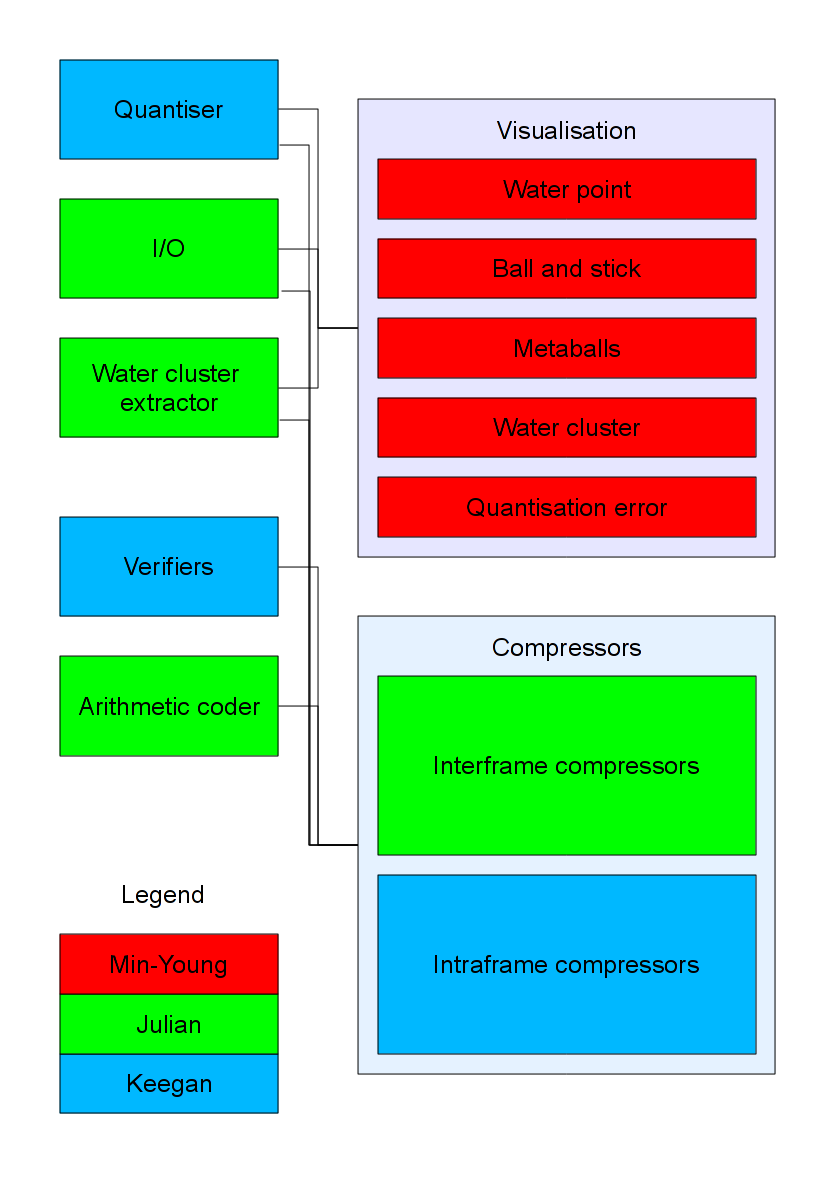
\includegraphics[width=100mm]{breakdown}
  \end{center}
  \caption{Overview of components within the system}
  \label{fig:design_overview}
\end{figure}

% }}}

\section{Visualisation}
% {{{
\label{sec:design_visualisation}

% {{{

The visualisation component is divided into a number of sub-components, which
are the different visualisation techniques chosen:

\begin{itemize}
  \item Water point visualisation
  \item Ball and Stick visualisation
  \item Metaballs visualisation
  \item Water cluster visualisation
  \item Quantisation error visualisation
\end{itemize}

% }}}

\subsection{Water point visualisation}
% {{{
\label{sub:design_waterpoint}

This visualisation technique is the simplest of all the visualisation
techniques in the system. A single point will be rendered per water molecule,
non-water molecules will be filtered out. Filtering out the non-water molecules
is the first step in reducing visible clutter. Using a low alpha value per
point further reduces clutter by causing areas with few overlapping points to
be more less visible, in comparison to areas with many overlapping points;
hence emphasising the areas with many overlapping points.

The advantage of this visualisation technique is that it allows for the larger
areas of water to be easily identified, however, the details are hidden.

% }}}

\subsection{Ball and stick visualisation}
% {{{
\label{sub:design_ballstick}

The ball and stick visualisation technique is used to provide more visual
information about the water molecules, the individual atoms of the water
molecules are visible. Rendering the individual atoms allows for the
orientation the water molecules to be seen.

As rendering all the water molecules will cause much clutter, the number of
molecules to render can be limited.

% }}}

\subsection{Metaballs visualisation}
% {{{
\label{sub:design_metaballs}

The metaballs technique is an alternative way to visualise the water volume in
the molecular simulation. The aim of the metaballs technique is to clearly
separate the areas of water, from the non-water areas. A surface is rendered
between the water and non-water areas of the volume.

To decrease the rendering cost of the surface, the surface is decimated.
Decimating the surface will simplify the surface, hence decrease the time
required to render it, and allow the volume to be more easily explored.

An alternative to decimating the surface in order to decrease the surface
complexity, is to decrease the amount of sampling done. Sampling the volume
less results in fewer triangles, but the surface quality will also decrease.

Decimation is preferred to decreasing the sampling amount as the surface
quality can be maintained. The render cost is decreased in exchange for
computation cost, where the computation is performed once for every frame.

% }}}

\subsection{Water cluster visualisation}
% {{{
\label{sub:design_watercluster}

The water molecules in a body of water is not completely uniform in all
directions, instead the water molecules form clusters. The compressors use this
knowledge to perform prediction, and thus it is useful to visualise these water
clusters.

To cope with the large number of water clusters that are present, the number of
clusters to render can be limited. Specific water clusters can also be rendered.

This visualisation technique is primarily useful in supporting the compression
aspect of the system. There has not been much emphasis on water clusters in
chemistry, thus it is unlikely that this visualisation technique will be of
interest to chemists.

% }}}

\subsection{Quantisation error visualisation}
% {{{
\label{sub:design_quanterror}

Quantisation is the only lossy step of the compression, thus it is important to
measure the amount of error that is introduced. To visually depict the
quantisation errors, the water molecules are coloured according to a colour
gradient. Water molecules with high quantisation errors are coloured so that
they are more visible and stand out, while water molecules with low
quantisation errors will be less visible.

This visualisation technique is only useful in supporting the compression aspect
of the system.

% }}}

% }}}

% }}}

